%!TEX root = paper.tex

\subsection{Concretization}

We have discussed Spack's internal software DAG model, and we have shown
how the spec syntax can be used to quickly specify a partially constrained
software DAG.  We say such a DAG is {\it abstract}, as it could potentially
describe more than one software configuration. Before Spack builds a spec, it
must ensure the following conditions:
\begin{enumerate}
\item No package in the spec DAG is missing dependencies.
\item No package in the spec DAG is virtual.
\item All parameters are set for all packages in the DAG.
\end{enumerate}
If a spec meets all of these criteria, we say it is {\it concrete}.
{\it Concretization} is the central component of the Spack build
process that allows it to reduce a highly unconstrained abstract
description to a concrete build.

\begin{figure*}
	\centering
	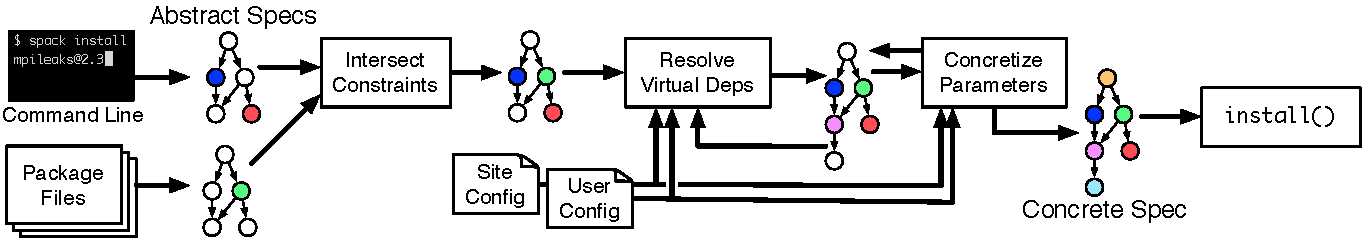
\includegraphics[width=\textwidth]{figs/concretization.pdf}
	\caption{
		Spack's concretization process.
		\label{fig:concretization}
	}
\end{figure*}

Spack's concretization algorithm is shown in Figure~\ref{fig:concretization}.
The process starts when a user invokes {\tt spack install} and requests that a
spec be built.  Spack converts the spec to an abstract DAG.
It then builds a {\it separate} spec DAG for any constraints that are encoded
in directives in package files. 

Spack intersects the constraints of the two DAGs package by package.  It checks
each parameter for inconsistencies.  Inconsistencies can arise if, for example,
the user inadvertently requests two versions of the same package, or if a
package file explicitly requests a different version from what the user requested.
Likewise, if the package and the user specified different compilers, variants,
or platforms for particular packages, this will cause the user to be notified
of the contradiction. If the user or package specified version ranges, they are
intersected, and if the ranges do not overlap, an error will be raised.
When the intersection succeeds, Spack has a single spec DAG with the merged
constraints of the user and the package files.  

The next part of the process is iterative.
If any node in the DAG is a virtual dependency, spack replaces it with with a
suitable interface provider.  It does this by building a reverse
index from virtual packages to providers using the {\tt provides when} 
directives discussed in Section~\ref{sec:virtual}. If multiple providers
could satisfy the constraints on the virtual spec, 
Spack will consult site and user policies to select the ``best'' possible
provider.  The selected provider may {\it itself} have virtual dependencies,
so Spack repeats this process until there are no more virtual packages
in the DAG.

With the now non-virtual DAG, Spack again consults site and user preferences for 
variants, compilers, and versions to resolve any remaining abstract nodes.
Adding a variant {\it may} cause a package to depend on more libraries. For example,
if the site default behavior is to have a particular package build with {\tt +python},
and this causes it to depend on Python libraries, then the cycle begins again.
Spack currently avoids an exhaustive search by using a greedy algorithm.  
It will not backtrack to try other options if its first policy choice leads
to an inconsistency.  Rather, it will raise an error and the user must resolve
the issue by being more explicit.  The user might toggle a variant, or she might
force the build to use a {\it particular} MPI implementation
by supplying, e.g. \verb|^openmpi| or \verb|^mpich|.  In future
work we will investigate adding a SAT solver to Spack's concretization process
to present users with better options.  In our experience, however, complex policy
interactions like these are very rare.

When the concretization process completes, it outputs a fully concrete spec DAG. 
A concrete DAG with architectures, compiler, versions, and variants, and all 
dependencies resolved is shown in Figure~\ref{fig:specs-mpileaks-concrete}.
This fulfills Spack's guarantees.  

\begin{figure}
	\centering
	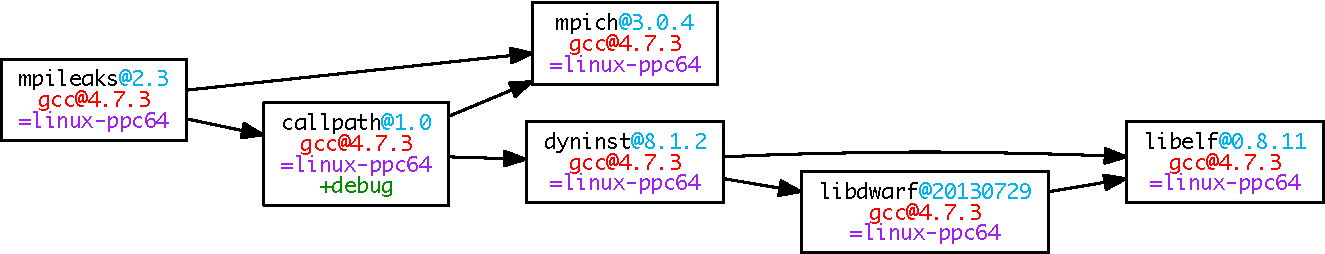
\includegraphics[width=\columnwidth]{specs/mpileaks-concrete.pdf}
	\caption{
		Concretized spec from Figure~\ref{fig:specs-mpileaks}.
		\label{fig:specs-mpileaks-concrete}
	}
\end{figure}

At install time, Spack constructs a package object for each node in the spec DAG
and traverses the DAG in a bottom-up fashion.  At each node, it invokes the package's
{\tt install} method.  For the {\tt spec} parameter to install, it uses a sub-DAG
rooted at current node, which is also a concrete spec.  Package authors are
responsible for querying the spec in {\tt install} and handling different configurations.

\subsubsection{Directory Layout}\label{sec:directory-layout}
\begin{figure}\centering
   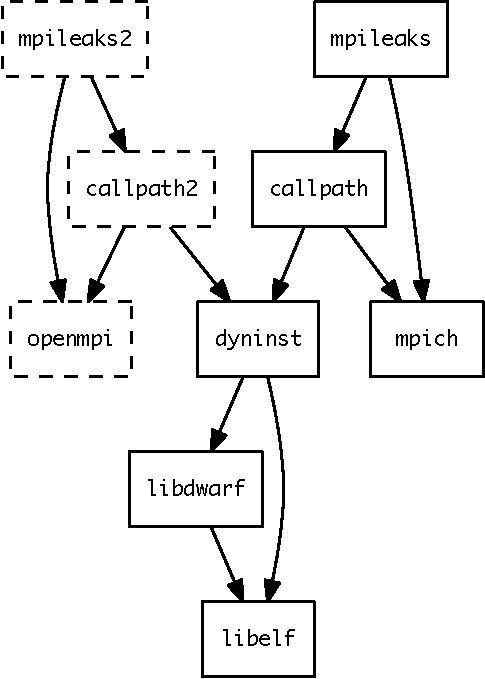
\includegraphics[width=\linewidth]{specs/rpaths.pdf}
   \caption{
       {\tt mpileaks} built with {\tt mpich}, then {\tt openmpi}.
       \label{fig:reuse}
   }
\end{figure}

We mentioned in Section~\ref{sec:packages} that each unique configuration is
guaranteed a unique install prefix. Spack uses the concrete {\it spec} 
to generate a unique path, shown in Table~\ref{tab:naming-conventions}.
To prevent the directory name from growing too long, Spack uses a SHA hash of
dependencies' specs as the last directory component.  This
does {\it not} mean that Spack rebuilds every library for each new configuration.
If two configurations share a sub-DAG, then the sub-DAG's configuration will
be reused.  Figure~\ref{fig:reuse} shows how the {\tt dyninst} sub-DAG is used for
both the {\tt mpich} and {\tt openmpi} builds of {\tt mpileaks}.


\subsubsection{Reproducibility}
For reproducibility and to preserve provenance, Spack stores a file containing
the concrete spec in each
install prefix. The spec can be examined later to understand how the installed
package was built.  It an also be used to reproduce the build on another machine
or at another site.

\subsubsection{Site policies and build complexity}

Our experience with manual installs helped us understand that much of the complexity
of building HPC software comes from the size of the build parameter space.  
As mentioned, there are only a few parameters most users care about, and the rest
only serve to add complexity to the build.  When doing manual builds, LLNL staff
tend to make arbitrary choices about many of the secondary build parameters,
or they would include logic in build scripts to make many of these choices.
In either scenario, publicly installed software was generally not installed
in a consistent way.

Concretization provides two benefits.  First, it allows users and staff to 
request builds with a minimal spec expression, while still providing a
mechanism for the site and the user to make consistent, repeatable choices about
other build parameters.  For example, the site or the user can set default versions
to use for {\it any} library that is not specified explicitly.
%
Second, concretization reduces the burden of packaging software because package authors
do not have to make these decisions.  There is no
need for packages to contain complicated checks, or for packages to be overly
specific about versions.  Other multi-configuration systems like Nix, EasyBuild,
and hashdist require the package author to write a mostly concrete build spec in advance.
We believe that this puts undue burden on the package author, and it makes the task
of changing site policies within a software stack difficult.  Spack
separates these concerns.























